\documentclass[
  % -- opções da classe memoir --
  article,			       % indica que é um artigo acadêmico
  12pt,				         % tamanho da fonte
  oneside,			       % para impressão apenas no recto. Oposto a twoside
  a4paper,			       % tamanho do papel. 
  % -- opções da classe abntex2 --
  %chapter=TITLE,		   % títulos de capítulos convertidos em letras maiúsculas
  %section=TITLE,		   % títulos de seções convertidos em letras maiúsculas
  %subsection=TITLE,	 % títulos de subseções convertidos em letras maiúsculas
  %subsubsection=TITLE % títulos de subsubseções convertidos em letras maiúsculas
  % -- opções do pacote babel --
  english,		       	 % idioma adicional para hifenização
  brazil,			      	 % o último idioma é o principal do documento
  sumario=tradicional
]{abntex2}


% ---
% Pacotes fundamentais 
% ---
\usepackage{lmodern}		        	% Usa a fonte Latin Modern
\usepackage[T1]{fontenc}      		% Selecao de codigos de fonte.
\usepackage[utf8]{inputenc}   		% Codificacao do documento (conversão automática dos acentos)
\usepackage{indentfirst}	      	% Indenta o primeiro parágrafo de cada seção.
\usepackage{color}				        % Controle das cores
\usepackage{graphicx}			        % Inclusão de gráficos
\usepackage{microtype} 			      % para melhorias de justificação
\usepackage{listings}

% \setlength{\cftsubsubsecindent}{0pt}% Remove indent for \subsubsection

% ---
% Pacotes adicionais, usados apenas no âmbito do Modelo Canônico do abnteX2
% ---
\usepackage{lipsum}				% para geração de dummy text
\usepackage{tocloft}
% ---
% Pacotes de citações
% ---
\usepackage[brazilian,hyperpageref]{backref}	 % Paginas com as citações na bibl
\usepackage[alf]{abntex2cite}                  % Citações padrão ABNT
% --- 
% CONFIGURAÇÕES DE PACOTES

% Configurações do pacote backref
% Usado sem a opção hyperpageref de backref
\renewcommand{\backrefpagesname}{Citado na(s) página(s):~}
% Texto padrão antes do número das páginas
\renewcommand{\backref}{}
% Define os textos da citação
\renewcommand*{\backrefalt}[4]{
	\ifcase #1 %
		Nenhuma citação no texto.%
	\or
		Citado na página #2.%
	\else
		Citado #1 vezes nas páginas #2.%
	\fi}%
% ---

% ---
% Retirar identação do sumário
% --- 
\newcounter{mysection}
\renewcommand\themysection{\Alph{mysection}}

% Writes the entry in the ToC with the required indentation
\newcommand\ToToC[1]{%
  \addcontentsline{toc}{section}   {\hspace*{4em}\appendixname~\themysection\hspace*{1em}#1}
}

\makeatletter
\newcommand\mysection{\refstepcounter{mysection}%
  \@startsection{paragraph}{4}{\z@}%
  {-3.5ex \@plus -1ex \@minus -.2ex}%
  {2.3ex \@plus.2ex}%
  {\normalfont\Large\bfseries}}
\renewcommand*\l@section{\@dottedtocline{1}{0em}{4em}}%
\renewcommand*\l@subsection{\@dottedtocline{2}{0em}{4em}}%
\renewcommand*\l@subsubsection{\@dottedtocline{3}{0em}{4em}}%
\newcommand*\l@mysection{\@dottedtocline{4}{1em}{1em}}%
\renewcommand\appendix{\par
  \setcounter{section}{0}%
  \setcounter{subsection}{0}%
  \renewcommand\theparagraph{\Alph{mysection}}
  \renewcommand\themysection{\@Alph\c@paragraph}}
\makeatother

\setcounter{secnumdepth}{4}
\setcounter{tocdepth}{3}
% ---
% 
% --- 

% ---
% Configurações do pacote backref
% Usado sem a opção hyperpageref de backref
\renewcommand{\backrefpagesname}{Citado na(s) página(s):~}
% Texto padrão antes do número das páginas
\renewcommand{\backref}{}
% Define os textos da citação
\renewcommand*{\backrefalt}[4]{
	\ifcase #1 %
		Nenhuma citação no texto.%
	\or
		Citado na página #2.%
	\else
		Citado #1 vezes nas páginas #2.%
	\fi}%
% ---
% ---
% Definindo formatação para exibição de código
% ---
\definecolor{codegreen}{rgb}{0,0.6,0}
\definecolor{codegray}{rgb}{0.5,0.5,0.5}
\definecolor{codepurple}{rgb}{0.58,0,0.82}
\definecolor{backcolour}{gray}{0.6}

\lstdefinestyle{mystyle}{
    commentstyle=\color{codegreen},
    keywordstyle=\color{magenta},
    numberstyle=\tiny\color{codegray},
    stringstyle=\color{codepurple},
    basicstyle=\ttfamily\footnotesize,
    breakatwhitespace=false,
    breaklines=true,
    captionpos=b,
    keepspaces=true,
    numbers=left,
    numbersep=5pt,
    showspaces=false,
    showstringspaces=false,
    showtabs=false,
    tabsize=2
}
\lstset{
  style=mystyle,
}
% ---
% 
% ---
\graphicspath{{../images/}}
% O tamanho do parágrafo é dado por:
\setlength{\parindent}{1.3cm}
% ---
% 
% ---
% Controle do espaçamento entre um parágrafo e outro:
\setlength{\parskip}{0.2cm}  % tente também \onelineskip
% ---
% 
% ---
% Espaçamento simples
\SingleSpacing
% ---
% Informações de dados para CAPA
% ---
\titulo{Uma Introdução a Haskell}
\autor{Gustavo Lopes Rodrigues \and Lucas Santiago \and Pedro Souza \and Thiago Henriques}
\local{Belo Horizonte}
\data{2020}
\instituicao{%
  Pontifícia Universidade Católica Minas Gerais
  }
\tipotrabalho{Trabalho de LIP}
% ---
% 
% ---
% informações do PDF
\makeatletter
\hypersetup{
     	%pagebackref=true,
		pdftitle={\@title}, 
		pdfauthor={\@author},
    	pdfsubject={Trabalho de Linguagem de programação em LaTeX},
	    pdfcreator={GLR, LSO, PS, THN},
		pdfkeywords={abnt}{latex}{abntex}{abntex2}{Linguagem de programação}, 
		colorlinks=true,       		% false: boxed links; true: colored links
    	linkcolor=black,          	% color of internal links
    	citecolor=blue,        		% color of links to bibliography
    	filecolor=magenta,      		% color of file links
		urlcolor=blue,
		bookmarksdepth=4
}
\makeatother
% ---
% Iniciando efetivamente o documento
% ---
\begin{document} 

    % Fazer com que as secções sejão subcapitulos
    \renewcommand{\thesection}{\noindent\arabic{chapter}.\arabic{section}}. 
    % ---
    % Selecionando linguagem
    % ---
    \selectlanguage{brazil}
    % ---
    % Retira espaço extra obsoleto entre as frases.
    % ---
    \frenchspacing
    % ---
    % Imprimir a capa 
    % ---
    \imprimircapa
    % ---
    % Imprimir a tabela de conteúdos(Sumário)
    % ---
    \pdfbookmark[0]{\contentsname}{toc}
    \tableofcontents*
    \cleardoublepage
    % ---
    % PARTE TEXTUAL
    % ---
    \textual
    % ---
    % Criar nova página e então iniciar a escrita
    % ---
    \newpage
    \chapter{Introdução}

    Em 1930, Alonzo Church , matemático estadunidense apresentou o Cálculo Lambda, como parte da investigação dos fundamentos da matemática. O Cálculo Lambda é um sistema que
    estuda funções recursivas computáveis, e foi utilizada como base para as teorias e fundamentos matemáticos por trás do paradigma da Programação Funcional. Ele também
    pode ser considerado a primeira linguagem programação funcional, todavia, não foi projetada para ser executada em computadores, sendo apenas um modelo que descreve relações entre funções
    simples, permitindo criar funções mais complexas.

    Com o passar dos anos, varias linguagens funcionais foram criadas, sendo alguns exemplos a linguagem LISP em 1955 e a ML no final da década de 70. Porém, não
    havia um padrão para as linguagens desse paradigma, e quando chegou a segunda metade da década de 80, havia uma necessidade para criar uma única linguagem, que englobasse
    as melhores práticas de projeto, além de implementar as técnicas funcionais que estavam em alta na época.

    Nesse contexto Haskell foi criado em 1987, por Peyton Jones e Paul Hudak. Sendo assim a The Yale Meeting foi a primeira reunião presencial , no qual foi decidido
    os principais objetivos que a linguagem proporcionaria, como também a escolha do nome. 
    Segue as metas estabelecidas na reunião:

    \begin{itemize}
      \item Ser viável para o ensino, pesquisa e aplicações, incluindo sistema de larga escala;
      \item Ser completamente descritiva via publicação no tocante à sua sintaxe e sua semântica;
      \item Não ser proprietária, tal que qualquer um pudesse implementá-la e distribuí-la;
      \item Basear-se em ideias que envolvessem o senso comum;
      \item Reduzir a diversidade desnecessária de outras linguagens funcionais.
    \end{itemize} 

    A implementação de Haskell começou do zero, desenvolvendo funções únicas e tendo inspiração na linguagem Miranda que estava desempenhando um papel 
    importante na época. Em geral, essa linguagem passou por algumas versões que ajudou muito no desempenho e na adição de novas funções. 

    \newpage
    \chapter{Histórico sobre a linguagem, com sua cronologia}

    Depois desse evento, outras reuniões se sucederam e sendo assim no dia 01/04/1990, foi publicado primeiro relatório
    da versão 1.0 do Haskell. Durante os proximos 15 anos, Haskell teve o lançamento de diferentes versões, tranzendo outras
    funcionalidades para linguagem, entre elas se encontra Haskell'98 e Haskell 2010 que é a versão mais recente de Haskell.  

    O relatório da versão do Haskell'98 foi lançado em fevereiro de 1999. Ela surgiu no intuito de estabeler uma versão mais estável, 
    para ser possível realizar a documentação mais profunda da lingua em livros, já que o Haskell estava evoluindo muito rápido e ganhando 
    notoriedade.

    Em 2006 a equipe começou a planejar revisões anuais para adicionar o progresso do desenvolvimento da linguagem. Sendo assim a primeira revisão,
    publicada em julho de 2010, foi nomeada Haskell 2010 e nela foi incrementada uma serie recursos que antes não estavam disponiveis.
    Segue abaixo uma serie dos recursos que foram disponibilizados:
    
    \begin{itemize}
      \item Do and If Then Else 
      \item Hierarchical Modules
      \item Empty Data Declarations
      \item Fixity Resolution 
      \item Foreign Function Interface
      \item Line Comment Syntax
      \item Pattern Guards
      \item Relaxed Dependency Analysis
      \item Language Pragma
      \item Remove n+k patterns
    \end{itemize}

    Atualmente existem 3930 programadores com contas registradas que utilizam Haskell, sendo que 2566
    dessas contas são publicas e 1364 privadas. Por causa do número de programadores existem muitas 
    oportunidades nessa área, fazendo os empregos terem um sálario médio de \$80K à \$160K.

    Por mais que Haskell não seja tão utilizado como antes, muitos aplicações foram feitas com a linguagem. 
    Algumas aplicações são:

    \begin{itemize}
      \item A biblioteca open-source Semantic, implementada pelo GitHub, foi puramente escrito em Haskell.
      \item O Facebook implementa programas anti spam que são escritos e Haskell e são de código aberto.
      \item O Snap e Yesod, ambos frameworks para aplicações na web, foram feitos para suportar Haskell.
      \item O Linspire, sistema operacional comercial, tem Haskell como linguagem escolhida para o desenvolvimento das ferramentas no sistema.
      \item Xmonad, totalmente escrito em Haskell, é um gerenciador de janela para o sistema X Window System
    \end{itemize}

    \begin{figure}[ht]
      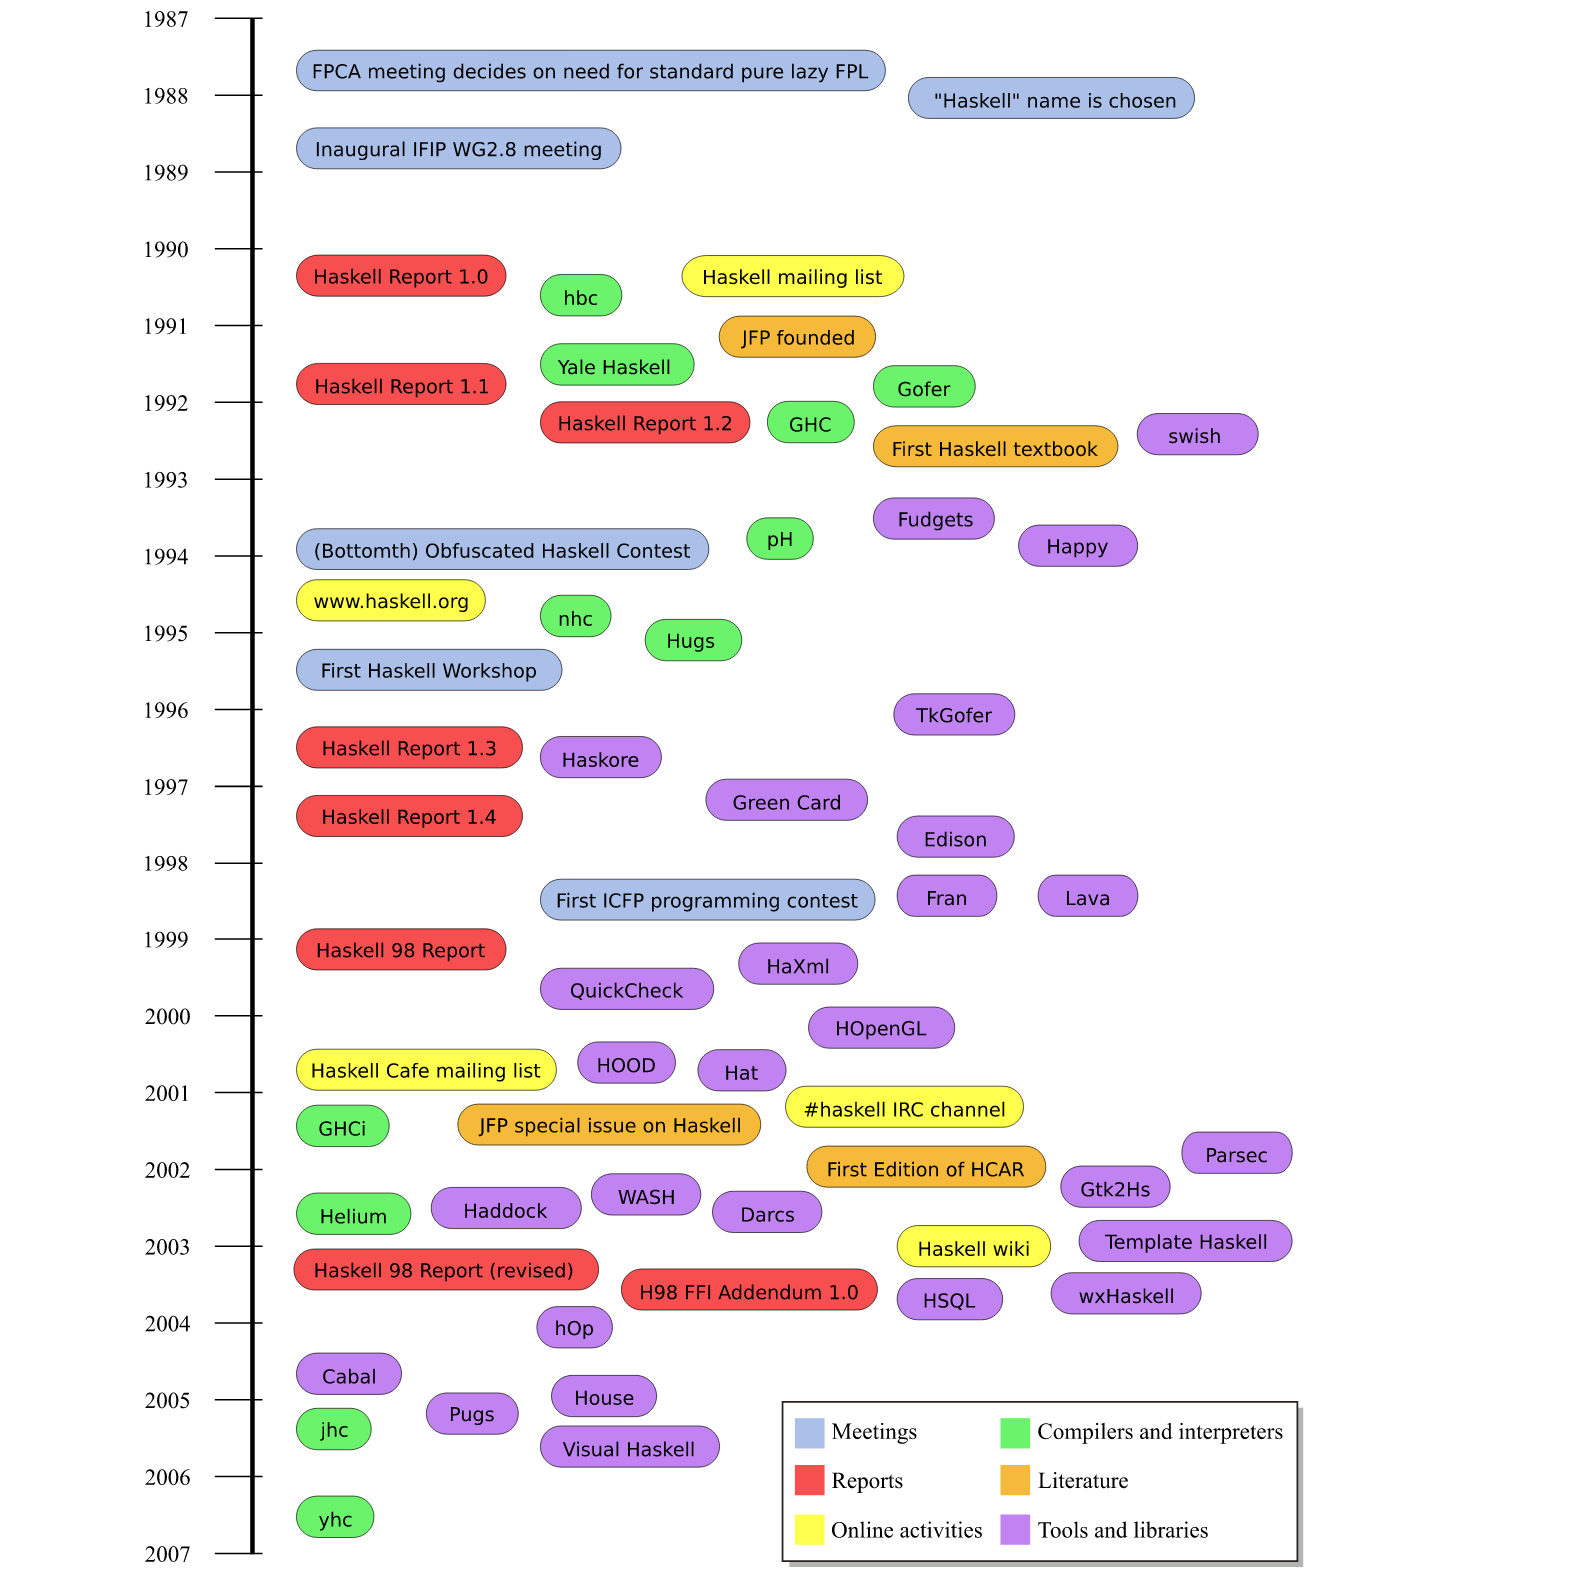
\includegraphics[width =\textwidth]{timeline.png}
      \caption{Cronologia do Haskell}
    \end{figure}

    \newpage

    \chapter{Paradigma a que pertence}

    O paradigma oferece e determina a visão que o programador possui sobre a estruturação
    e a execução do programa. Um exemplo bem famoso de paradigma é o POO ( Programação orientada a objetos).
    Já a Programação funcional é um paradigma que descreve uma expressão matemática a ser avaliada,
    mapeando dos valores de entradas nos valores de retorno, por meio de funções. Em outras palavras: 
    a programação funcional só funciona em cima de funções.

    Eis mais algumas características do paradigma
    \begin{itemize}
      \item Dados imutáveis e são evitados estados. 
      \item Não existe efeitos colaterais 
      \item "Funções puras" (sem efeitos colaterais)
      \item Cálculo Lambda
    \end{itemize}

    \newpage

    \chapter{Características mais marcantes da linguagem}

    \begin{itemize}
      \item Como dito anteriormente, a linguagem só faz utilização de funções e funções dentro de funções. Por isso
      Haskell é descrito como puramente funcional.
      \item Haskell possui uma sintaxe simples, elegante e concisa. Como resultado, programas em Haskell possuem 
      poucas linhas. 
      \item Além disso, a linguagem usa avaliação preguiçosa(Lazy evaluation), que é uma técnica para atrasar a computação 
      até um ponto em que o resultado da computação é considerado necessário.
      \item Tipagem estática: Verificação dos tipos usados em dados e variáveis para 
      garantir que sempre está sendo usado um tipo que é esperado em todas as situações. 
      \item função de ordem superior: Função que tem como argumento uma outra função, ou que produz 
      uma função como resultado.
    \end{itemize}

    \newpage 

    \chapter{Linguagem similares ou confrontantes}

    \begin{itemize}
      \item Prolog
      \item LISP 
      \item Scheme 
      \item ML 
      \item Miranda 
      \item Elixir 
    \end{itemize}

    \newpage

    \chapter{Exemplo(s) de programa(s)}

    \section{Hello World em Haskell}
      \lstinputlisting[language=haskell]{helloworld.hs}

    \section{Quicksort}
      \subsection{Exemplo de Quicksort em C}


      \lstinputlisting[language=c]{quicksort.c}
      \subsection{Exemplo de Quicksort em Haskell usando compreensão de lista} 

      \lstinputlisting[language=haskell]{quicksort_list.hs}      

      \subsection{Exemplo de Quicksort em Haskell usando a função filter}

      \lstinputlisting[language=haskell]{quicksort_filter.hs}

      \section{Explicação dos algoritmos}
      Os algoritmos em Haskell são extremamente compactos em relação à C. Sua sintaxe não tem foco
      em programar diretamente a memória, como acontece em C. Começando pelo \emph{Hello World} simples que possui ou evoluindo
      para um quicksort, a lingua mostra-se bem compacta e direta na resolução dos problemas.

      No primeiro exemplo, foi usado \emph{list comprehension} para resolver o problema. Na primeira linha,
      foi declarado uma lista vazia para ser retornada caso o quicksort receba uma lista sem valores. A segunda linha
      cria uma função recursiva, caso tenha valores na lista para serem ordenados.

      \subsection{Exemplo de Quicksort em Haskell usando a função filter}

      \lstinputlisting[language=haskell]{quicksort_c2haskell.hs}
      
      Esse é um modelo traduzido diretamente do exemplo do quicksort em C para Haskell. Modelo resumido usando recursos da linguagem
      abaixo:

      \subsection{Exemplo de Quicksort em Haskell usando a função filter resumido} 

      \lstinputlisting[language=haskell]{quicksort_c2Haskellresumido.hs}

      Mesmo resumindo o código a forma imperativa para o quicksort não parece ser uma boa opção, usar o quicksort de forma recursiva
      dentro do haskell torna o código muito mais simples e intuitivo.

    \newpage

    \chapter{Considerações finais}

    \newpage

    \postextual

    \bibliography{abntex2-modelo-references}
    \begin{apendicesenv}
      
        \partapendices

        %Corrigir erro da numeração dos apendices
        \setcounter{chapter}{0}
        \renewcommand{\thechapter}{\Alph{chapter}}%

        \chapter{Gustavo Lopes}

        O que eu achei de Haskell? Como um usuário de longa data de linguagens orientadas a objeto(OOP), 
        como Java, C++ e mais recentemente Dart, minha experiência inicial com Haskell foi...
        um pouco estranha. Fiquei muito curioso e até encucado em ver Haskell executar códigos, que em
        outras linguagens precisariam ocupar 50 linhas, em apenas 2 ou 3 linhas, como foi o Quicksort.

        Além disso, lendo sua história, achei extremamente fascinante toda a concepção do Haskell,
        mas fiquei até triste, vendo que é muito difícil encontrar muitas pessoas falando sobre essa linguagem, que nasceu 
        do esforço coletivo de vários programadores, mas que hoje não recebe tanto apoio como outras linguagens.

        Por fim, como curiosidade, eu estava procurando sobre como fazer interfaces em C++ quando
        descobri que a WxWidgets, uma biblioteca para criar interface cross-platform, também possui 
        sua versão para Haskell, chamada WxHaskell.

        \begin{figure}[ht]
          \includegraphics[width =\textwidth]{gebob.png}
          \caption{GeBoP, um jogo de tabuleiro feito em Haskell, usando WxHaskell}
        \end{figure}

        \newpage
        
        \chapter{Thiago Henriques}

        \newpage 

        \chapter{Lucas Santiago}

        Na minha opinião, Haskell se apresenta de uma forma muito diferente da maioria da outras línguas. 
        Parafraseando Fábio Akita: Cada língua de programação não é mais do que uma ferramenta
        para resolver um problema. 

        \begin{figure}[ht]
          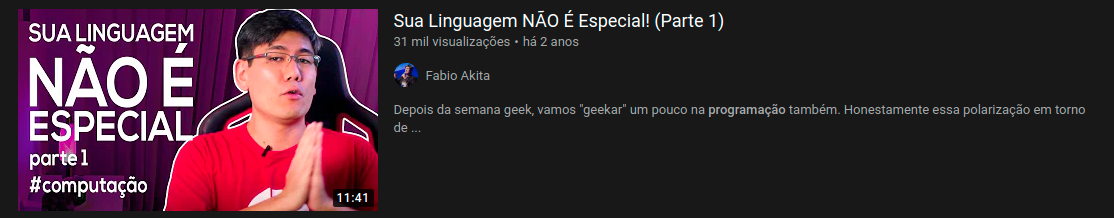
\includegraphics[width =\textwidth]{fabio_akita_lingua.png}
          \caption{\href{https://www.youtube.com/watch?v=p9-WuJbVHHc}{Fábio Akita explicando que linguas de programação são apenas feitas para resolver problemas!}}
        \end{figure}

        Os problemas que Haskell se propôs a resolver são cálculos matemáticos
        funcionais. O paradigma funcional dessa língua torna ela bem resistente a efeitos colaterais. Além de ser uma língua
        \emph{cross-platform}, extremamente importante para todas aquelas pessoas que precisem de uma língua que funcione
        em qualquer sistema operacional. 

        Como um programador de C/C++ e Python, vejo que Haskell está em um nível intermediário entre essas línguas.
        É interessante ver uma língua de alto nível com tipagem estática, torna o código bem estável - chances baixas de 
        resultar em erros -, tipagem é fundamental quando se quer garantir precisão de valores e tipos nos cálculos.

        Concluindo, não foi tão intuitivo aprender Haskell, ele possui várias propriedades que não existem em nenhuma das línguas
        que conhecia. Entretando, isso foi extremamente positivo para mim, aprendi várias coisas novas. Abaixo há
        mais um vídeo do Fábio Akita, dessa vez citando que nem sempre é fácil aprender algo novo. Em programação,
        quando você aprende da forma correta, várias novas possibilidades de resolução de problemas começam a aparecer.

        \begin{figure}[ht]
          \includegraphics[width =\textwidth]{fabio_akita_programar_eh_dificil.png}
          \caption{\href{https://www.youtube.com/watch?v=V7oUDL7E1g4}{Fábio Akita explicando que programação nem sempre é fácil.}}
        \end{figure}

        \newpage

        \chapter{Pedro Souza}

    
    \end{apendicesenv}

\end{document}


